\section{Energy efficiency}
As in exercise 1, when discussing energy efficiency, we will be focusing on amperage, since it's more relateable to, among other things, battery capacity.

\subsection{Readings}

In the final iteration of our implementation, we were able to have the microcontroller enter energy mode 4 with no extra peripherals enabled, allowing it to idle at about $2\mu A$. Figure \ref{idle-fig} shows a log-scale plot of the amperage while idle and figure \ref{playing-fig} shows the active amperage.

\begin{figure}[h!]
    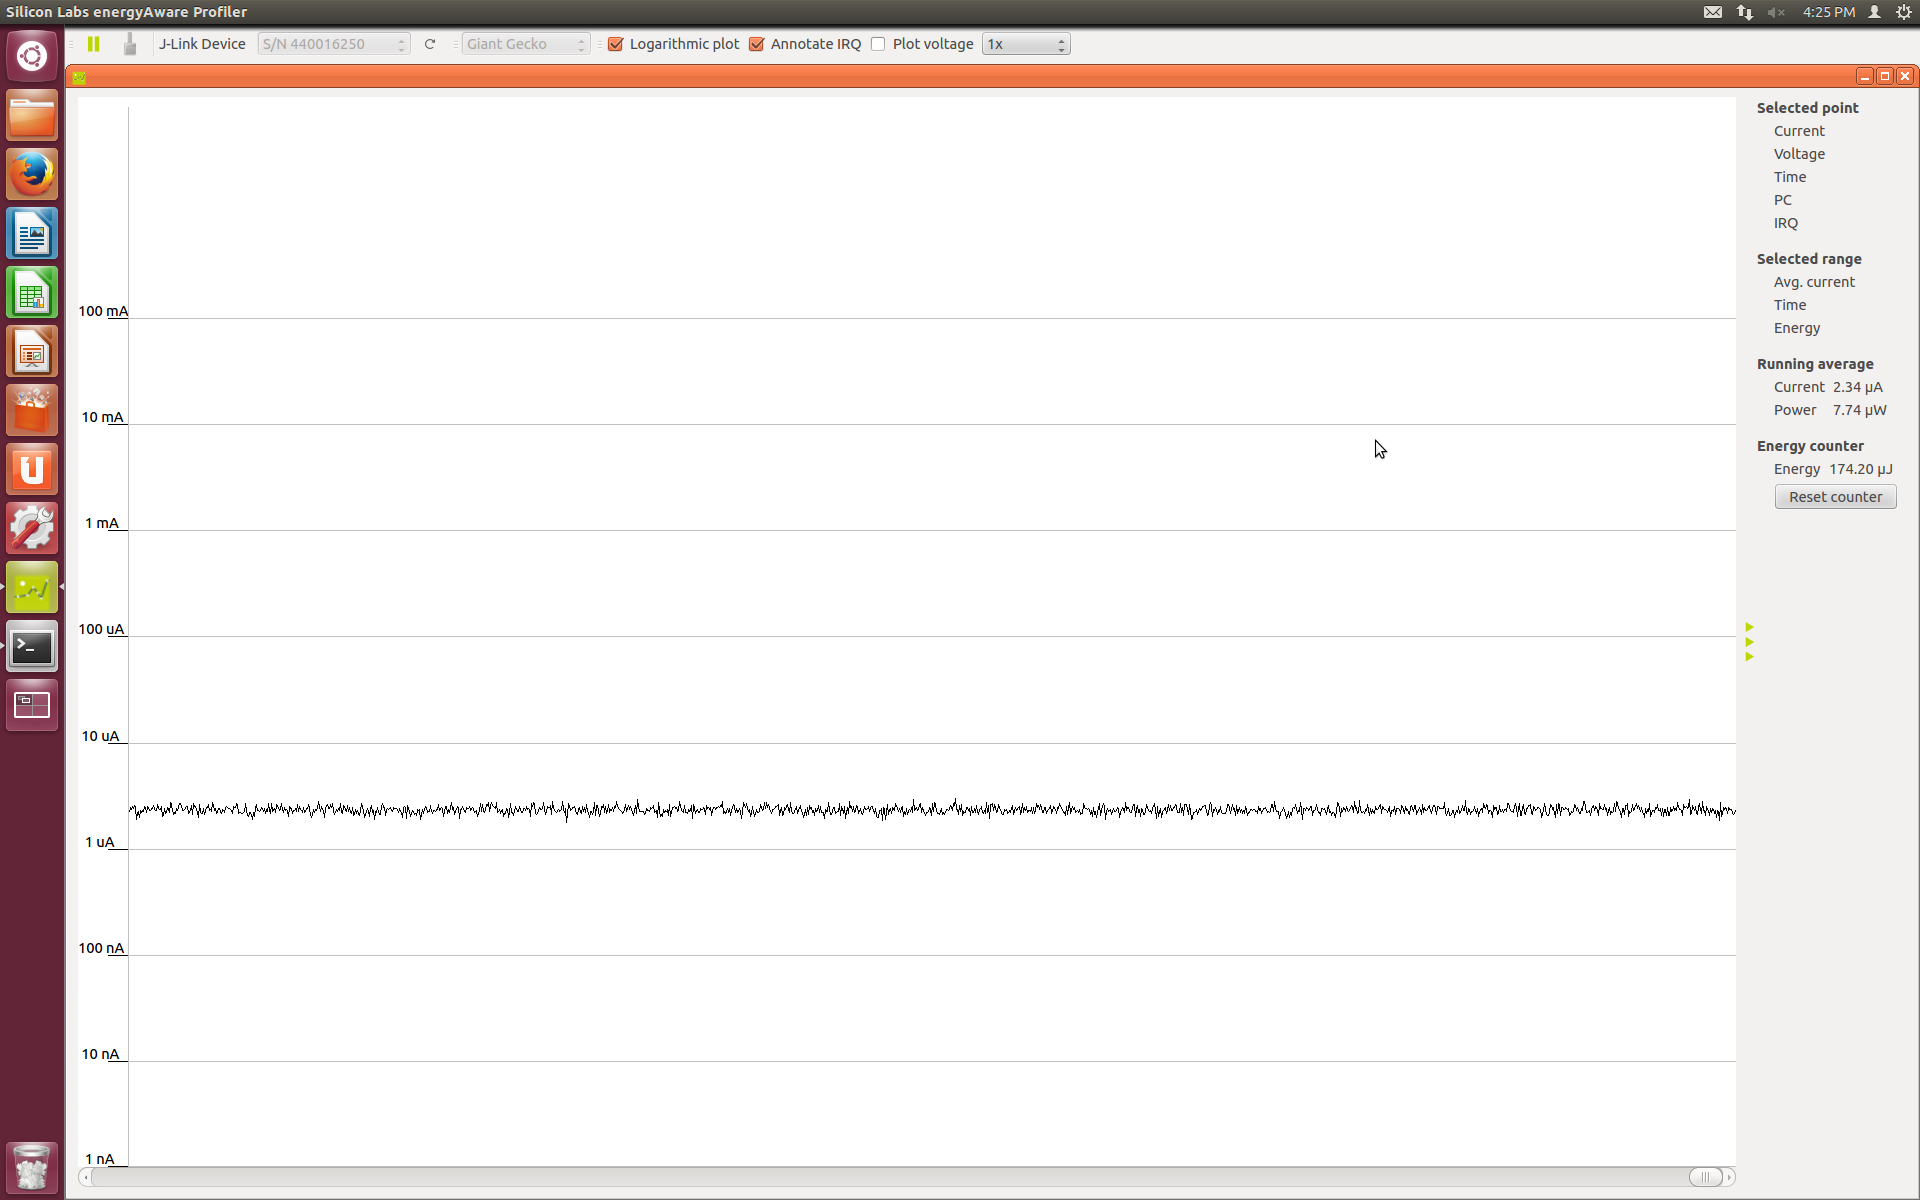
\includegraphics[width=\linewidth]{img/idle.png}
    \caption{Idle amperage plotted by the eAProfiler tool.}
    \label{idle-fig}
\end{figure}

\begin{figure}[h!]
    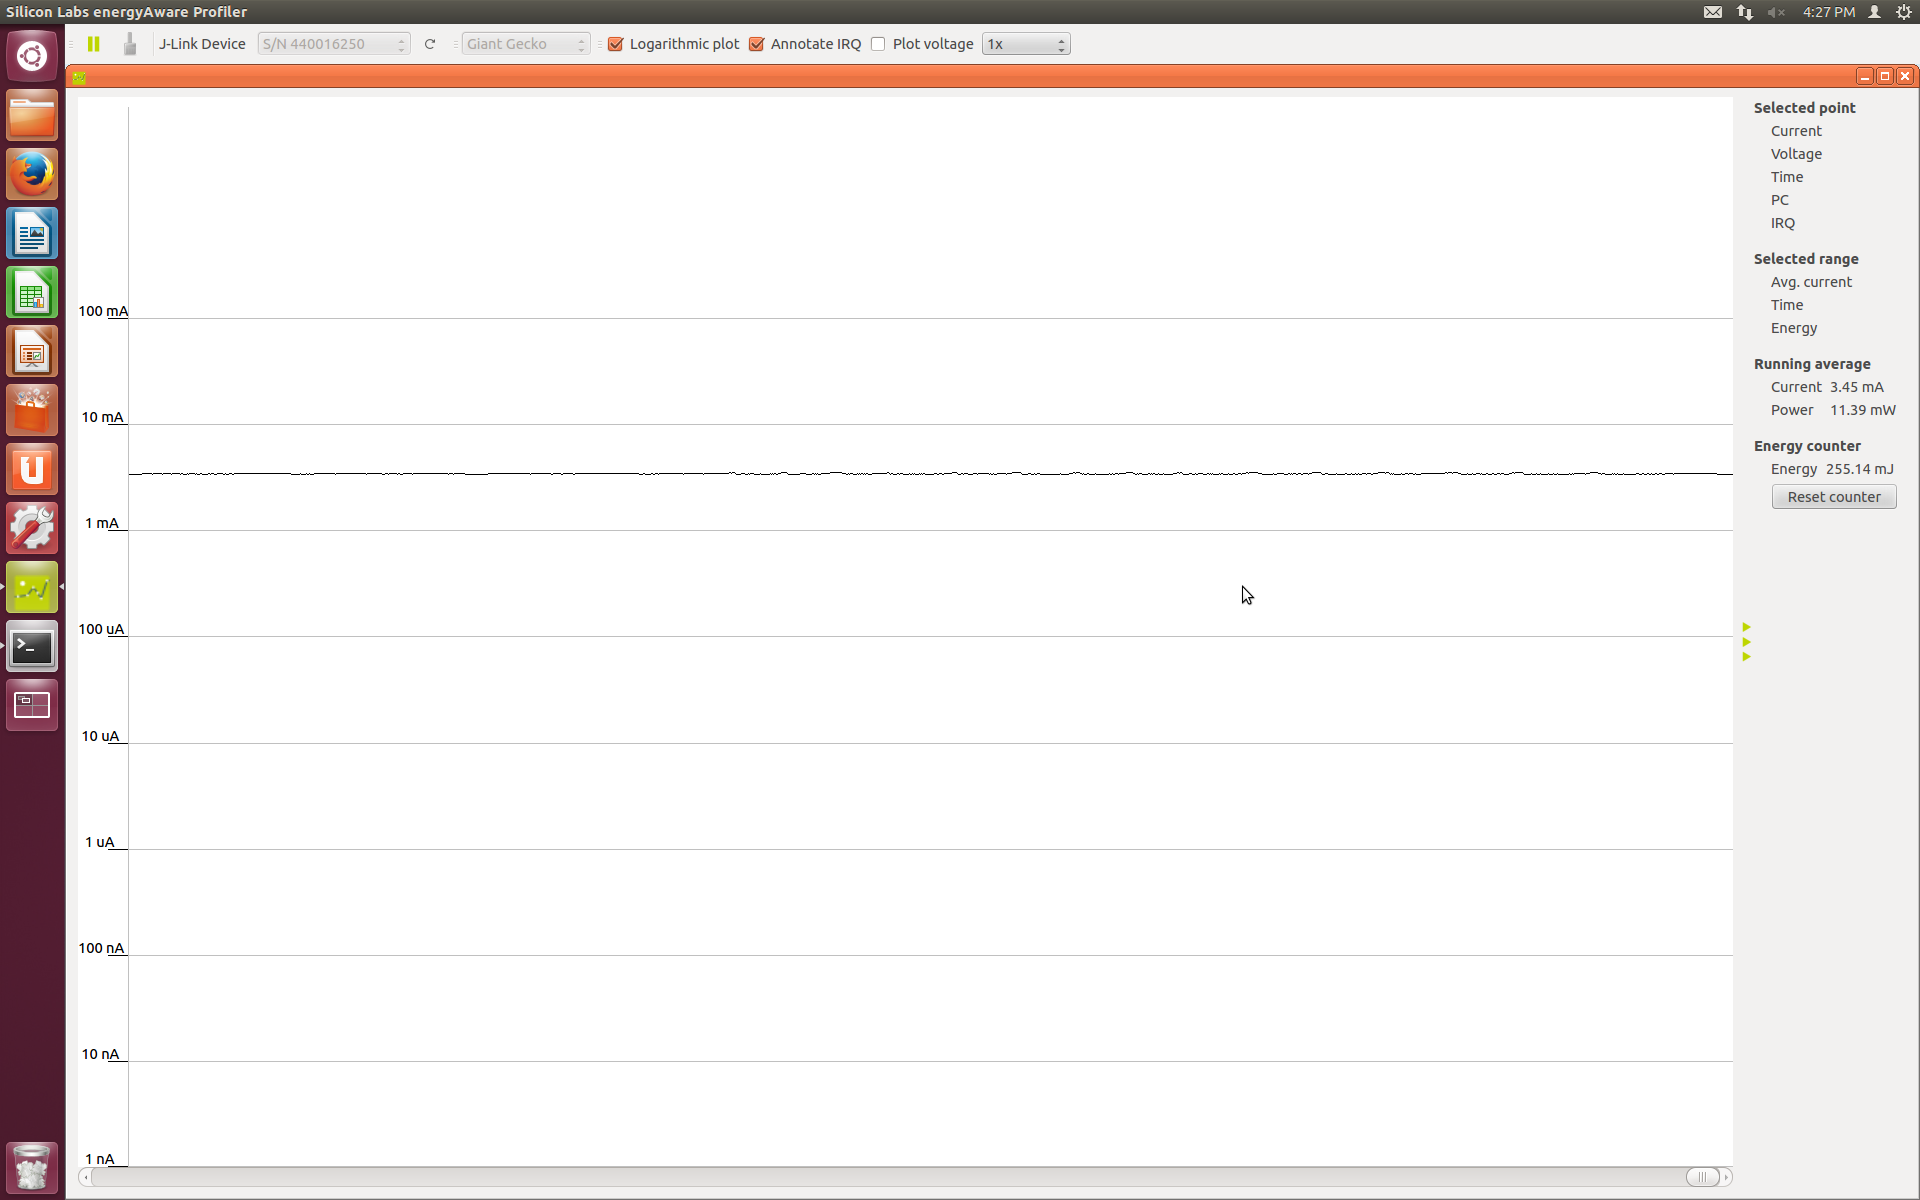
\includegraphics[width=\linewidth]{img/playing.png}
    \caption{Active amperage plotted by the eAProfiler tool.}
    \label{playing-fig}
\end{figure}

\subsection{Expected lifetime on a CR2032 battery}

In our report for exercise 1, we used the CR2032 battery as an example in the energy efficiency section. \cite[p.~13]{exercise1report} Since our idle power consumption is at the same level in this exercise as in the previous, our conclusion from that report still stands; in idle mode, the battery will deteriorate before discharging from the microcontrollers usage. This time however, the functionality of our program is rather different, and it spends a larger amount of time not idling. As can be seen from figure \ref{playing-fig}, the amperage while playing is around $3.5mA$. Using the same reference battery capacity \cite{cr2032} as in exercise 1, and the playing amperage, formula \ref{playing-formula} gives us an expected lifetime with continuous playing, of about 2 days, 20 hours.

\begin{gather}
\label{playing-formula}
\frac{240mAh}{3.5mA} = 68.6 hours
\end{gather}
